\documentclass[12pt,a4paper]{article}
\usepackage[paper=portrait,pagesize]{typearea}
\usepackage[left=2cm, right=2cm]{geometry}
\usepackage[utf8]{inputenc}
\usepackage[hidelinks]{hyperref}
\usepackage{graphicx, indentfirst, array, lscape}
\graphicspath{ {./images/} }

\renewcommand\contentsname{Índice}
\renewcommand\refname{Referências}
\renewcommand{\listfigurename}{Lista de Figuras}
\renewcommand{\figurename}{Figura}

\title{
    \textbf{Licenciatura em Engenharia Informática e de Computadores} \vspace{5mm} \\
    \textbf{Queuality} \\ 
    Sistema de Gestão de Filas de Espera
}
\author{
    Joana Campos, A44792 \href{mailto:a44792@alunos.isel.pt}{a44792@alunos.isel.pt} 
    \and Nuno Cardeal, A44863 \href{mailto:a44863@alunos.isel.pt}{a44863@alunos.isel.pt}
    \and Carolina Couto, A44871 \href{mailto:a44871@alunos.isel.pt}{a44871@alunos.isel.pt} \\
    \\
    \textbf{Orientador:} Paulo Pereira \href{mailto:paulo.pereira@isel.pt}{paulo.pereira@isel.pt}
}

\begin{document}
\maketitle
\pagebreak
\tableofcontents
\thispagestyle{empty}
\listoffigures
\newpage
\pagenumbering{arabic}


\pagebreak
\section{Introdução}
Numa sociedade onde existe cada vez mais adesão a multitasking, estar preso numa fila de espera,
parado sem fazer nada, pode ser considerado uma perda de tempo. Tempo esse que poderia ser usado
para trabalhar ou para “ir beber um café”. Principalmente nestes tempos de pandemia estar em contacto
com outras pessoas deve ser evitado.\par

Para contornar esta situação, uma solução viável seria um sistema de gestão de filas de espera que,
assumindo que o cliente se encontra próximo do local onde espera ser servido, o notifica quando estiver
próximo da sua vez, evitando assim que o cliente tenha de estar presencialmente na fila, podendo ir
fazer outras coisas enquanto aguarda, melhorando assim a sua “qualidade de vida”.\par

Neste projeto pretende-se criar um sistema de gestão de filas de espera. O sistema incluirá a
autenticação dos funcionários para que possam realizar a gestão das diferentes filas. Terá ainda de
admitir a existência de pelo menos um administrador que estará encarregue de editar as filas de espera.
Os clientes terão a possibilidade de verem a senha atual de todas as filas, o número de senhas à sua
frente, retirar uma senha ou fazer marcação, e ainda, serão notificados quando a sua vez estiver próxima.\par 

\pagebreak
\section{Caracterização da Solução}
A solução deste projeto dividir-se-á em quatro partes, uma base de dados que irá guardar a
informação de cada utilizador, uma web API, uma aplicação web dirigida para os funcionários do
serviço e uma aplicação móvel dirigida para os clientes. 

A Web API divide-se em duas partes, a implementação das funcionalidades da aplicação e o
contrato público que disponibiliza as mesmas para as aplicações clientes. Como é possível ver na figura
1 a Web API será o elo de ligação entre as funcionalidades da nossa solução e a aplicação de cliente e
web. A implementação das funcionalidades irá ainda comunicar com a base de dados.

A aplicação web será destinada aos funcionários, sejam eles os que realizam o atendimento aos
clientes ou os que administram o sistema. Estes dois papéis são distintos uma vez que o primeiro estará
encarregue de avançar na fila de espera, e o último terá permissões para alterar o sistema das mesmas.

Para os clientes será disponibilizada uma aplicação móvel que permitirá obter a senha, conhecer
quantas senhas se encontram à sua frente, assim como receber notificações quando faltar um
determinado número de senhas para a sua vez.

\pagebreak
\section{Requisitos Funcionais}
\subsection{Base de Dados}
Nesta secção é apresentada a proposta de solução para a base de dados utilizada. Esta estará responsável
por armazenar a informação da Web API. No projeto presente a base de dados é não relacional, neste caso do tipo
\textit{Document Store} utilizando a tecnologia \textit{MongoDB} \cite{mongoDBReference}. A escolha deste tipo de base de dados deu-se ao 
facto de ser algo não muito explorado no curso e algo bastante usado na indústria. Base de dados do tipo documento
tem também como vantagem guardar os dados de forma bastante similhante aos objetos usados na aplicação em questão, reduzindo 
assim a necessidade de haver tradução dos dados como estariam guardados numa base de dados relacional para os dados que a aplicação recebe.
Na figura \ref{fig:figure1} encontra-se o modelo de dados utilizado neste projeto. Foi com base neste modelo que se criou as coleções e campos necessários para poder 
guardar a informação necessária.\par
\begin{figure}[h]
    \centering
    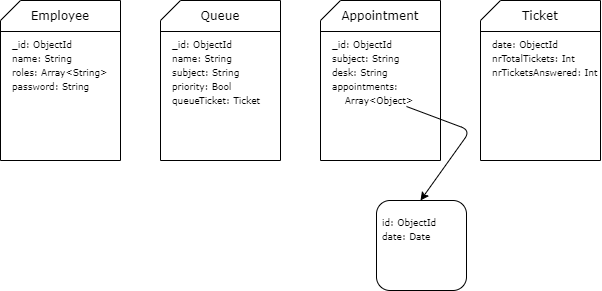
\includegraphics[scale=0.75]{Data-Model}
    \caption{Modelo de Dados do Queuality.}
    \label{fig:figure1}
\end{figure}
Começou-se por definir as coleções necessários para lidar com um sistema de gestão de senhas. Estas entidades ainda estão abertas para melhoramentos ou adição de campos
que se considerem necessários guardar. Assim, definiu-se a coleção \textit{Employee} \ref{fig:figure1} ilustrada na figura que irá conter a informação necessária para identificar um funcionário assim 
como os seus roles como funcionário da empresa em questão. Seguidamente, foi defenida a coleção \textit{Queue} ilustrada na figura \ref{fig:figure1} que irá conter o nome da fila, o assunto que irá ser tratado nessa fila
e também irá ser guardada a informação das senhas da fila em questão. A informação sobre as senhas de cada fila irá ser guardado num objecto definido por \textit{Ticket} em que irá conter o número de pessoas que foram atendidas
daquela fila, o número total de pessoas que tiraram senha naquela fila e finalmente a data que irá servir para reiniciar todos os dias a contagem das senhas a zero.
\subsection{Aplicação \textit{Web}}
Nesta secção é apresentada a proposta de solução para a aplicação \textit{web}. A aplicação web foi realizada com o propósito de ser utilizada pelos funcionários 
da empresa que usufruir do sistema em que irão ser englobadas diferentes ações a realizar, gerir as filas, gerir marcações realizadas e avançar nas senhas.
A aplicação irá ter um serviço de autenticação \textit{OpenId} para que apenas os funcionários autenticados possam realizar ditas ações.\par
Apesar de ainda não decidido, possivelmente os diferentes \textit{roles} que irão existir não poderão ter acesso a todos os links de navegação que 
irão estar disponíveis na aplicação \textit{web}.\par
Na aplicação escolheu-se usar a tecnologia \textit{React} \cite{reactReference} com \textit{TypeScript} \cite{typescriptReference}. A escolha de \textit{React}
para \textit{frontend} sucedeu-se visto que é uma tecnologia cada vez mais usada na indústria, é bastante simples de compilar e fácil e apresenta qualidade na \textit{user interface} 
o que é bastante importante para quem usufruir da aplicação. Para a linguagem estava-se indeciso entre \textit{JavaScript} ou \textit{TypeScript} acabando-se por escolher a última visto que
usa tipos o que consegues corrigir erros que poderia facilmente acontecer em JavaScript que é uma linguagem fracamente tipificada.\par
Neste momento todos os funcionários autenticados irão ter acesso à aplicação toda.\par
Na figura \ref{fig:figure2} está presente o diagrama de navegação utilizado para definir as diferentes páginas que a aplicação irá conter.
\begin{landscape}
    \begin{figure}
        \centering
        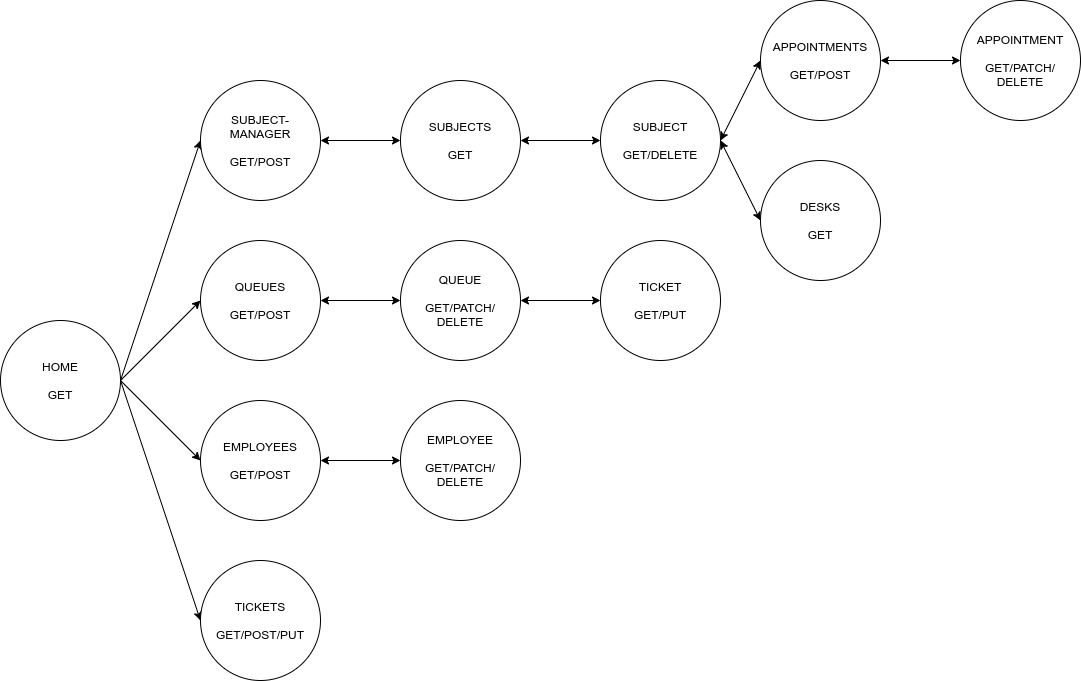
\includegraphics[scale=0.5]{Hypermedia-Navigation}
        \caption{Diagrama de navegação da Aplicação \textit{Web}}
        \label{fig:figure2}
    \end{figure}
\end{landscape} 
De seguida, desenhou-se a página de gestão das filas (\ref{fig:figure3}) em serão apresentados o nome das filas, o assunto das filas, a prioridade e onde
será possível editar, apagar e adicionar filas. Estas ações apenas aos funcionários que o papel designado para tal.\par
\begin{figure}[h]
    \centering
    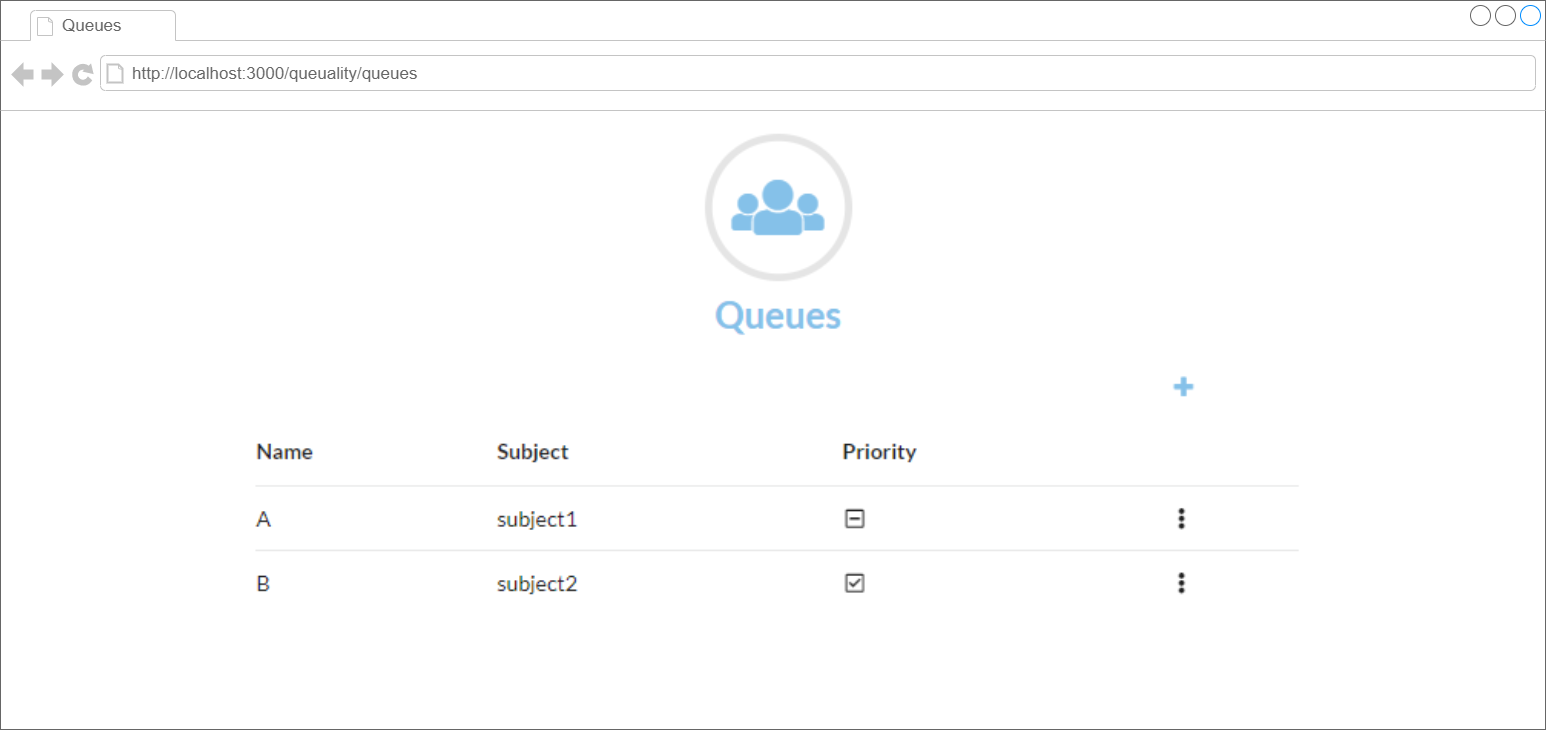
\includegraphics[scale=0.25]{QueuesMock}
    \caption{Mock da Aplicação \textit{Web}: Gestão das filas}
    \label{fig:figure3}
\end{figure}
Já na página dos tickets é possível visualizar as próximas cinco senhas a serem chamadas assim como o funcionário ter um botão em que lhe será possível avançar na
fila. Um \textit{mock} desta página encontra-se na figura (/ref{fig:figure4}).
\begin{figure}[h]
    \centering
    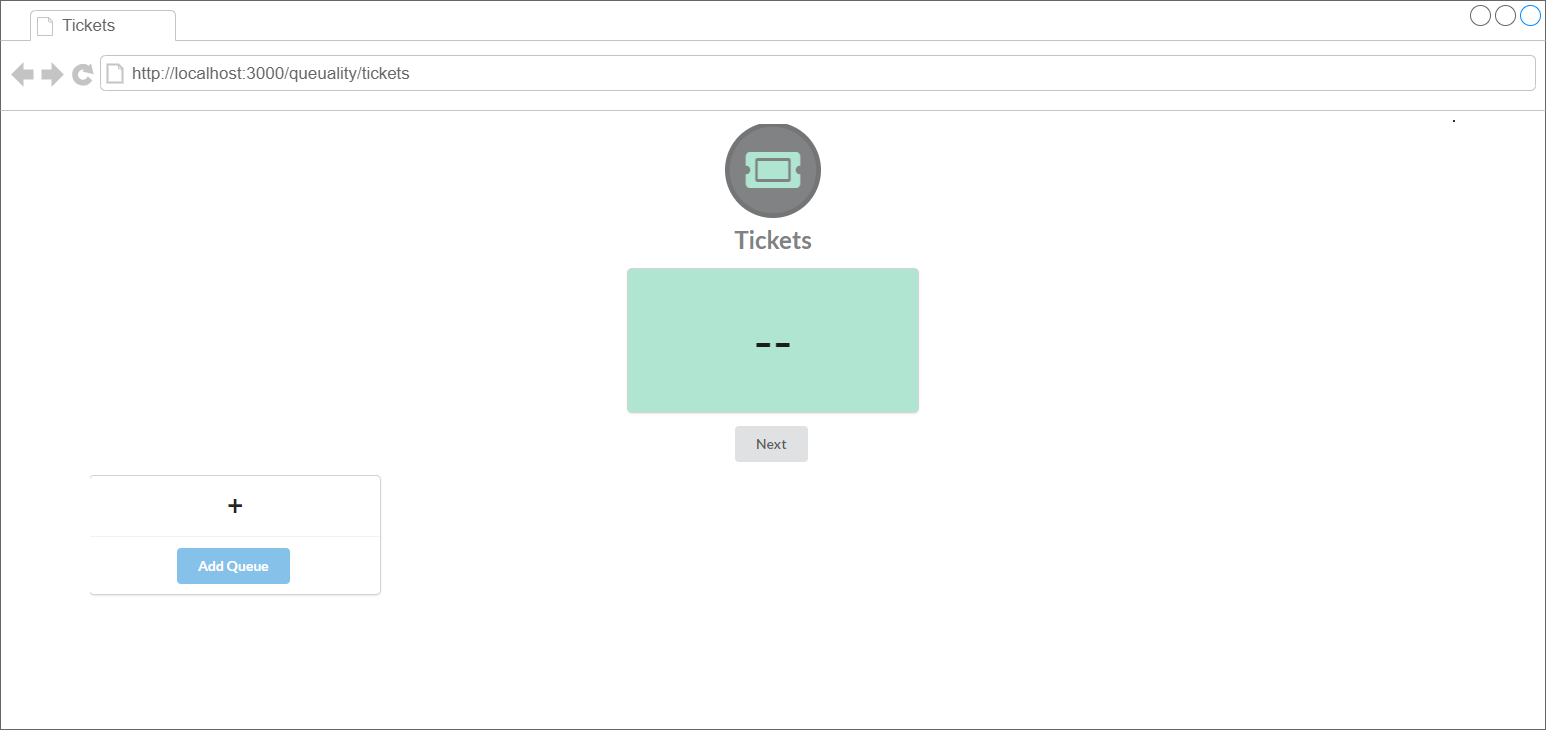
\includegraphics[scale=0.25]{TicketsMocks}
    \caption{Mock da Aplicação \textit{Web}: Gestão das senhas}
    \label{fig:figure4}
\end{figure}
\pagebreak
\subsection{Aplicação Móvel}
\pagebreak
\section{Requisitos Não Funcionais}
Para a solução deste projeto os recursos serão alocados numa base de dados não relacional, para dar
oportunidade ao aprofundamento dos conhecimentos sobre a mesma. Esta base de dados irá guardar os
utilizadores autenticados e as suas respetivas funções. Cada utilizador anónimo terá uma base de dados
local que guardará marcações e/ou senhas juntamente com a informação adicional que for necessária
no decorrer do projeto.
Tenciona-se realizar deployment na cloud de modo que o projeto tenha oportunidade de ser
distribuído a potenciais interessados. Terá a possibilidade de receber relatórios de análise de forma a
ser possível monitorizar os potenciais problemas que possam vir a ocorrer no sistema.
\pagebreak
\section{Estado atual do Projeto}
Neste momento, a componente servidora e a base de dados encontram-se implementadas, no entanto sempre prontas para melhoramentos. 
Em relação ao \textit{frontend}, na aplicação móvel, a atividade das filas encontra-se completa e a de o utilizador poder tirar uma senha 
também, ficando a faltar na sua totalidade as atividade das marcações. Em relação a aplicação web falta implementar a parte da autenticação,
a página da informação dos funcionários e a das marcações. Encontra-se completamente implementada a página das filas e a página das senhas 
encontra-se parcialmente implementada faltando apenas tomar algumas decisões finais.


\pagebreak
\begin{thebibliography}{9}    
    \bibitem{mongoDBReference} 
    MongoDB,\\\texttt{https://www.mongodb.com/}.
    Consultado a 15/04/2021
    \bibitem{reactReference} 
    React,\\\texttt{https://reactjs.org/}.
    Consultado a 10/03/2021    
    \bibitem{typescriptReference} 
    TypeScript,\\\texttt{https://www.typescriptlang.org/}.
    Consultado a 10/03/2021
\end{thebibliography}


\end{document}